\documentclass[8pt,conference,compsocconf]{IEEEtran}

\usepackage{geometry}
\geometry{margin=2cm,tmargin=2.2cm}
\usepackage{hyperref}
\usepackage{graphicx}	% For figure environment
\usepackage{xcolor}
\usepackage{amsmath}
\usepackage{amssymb}
\usepackage{booktabs}
\usepackage{dsfont}
\usepackage[caption=false]{subfig}
\usepackage{tabularx}
\usepackage{tikz}

\usepackage{multirow}


\begin{document}
\title{Project Report: Twitter Text Sentiment Prediction}

\author{
 Fereshte Mozafari, Mohammad Tohidi Vahdat, Ehsan Mohammadpour\\
 fereshte.mozafari@epfl.ch, mohammad.vahdat@epfl.ch, ehsan.mohammadpour@epfl.ch, \\
  \textit{EPFL, Switzerland}
}

\maketitle
\begin{abstract}
	Twitter sentiment Classification (whether they are positive or negative) have been studied in the recent years.
	In this work, we use a deep learning architecture to classify the sentiment of twitter messages. We use GloVe embedding to obtain feature representation for the messages. In the proposed model, we construct a long short-term memory recurrent neural networks with $4$ layers. The architecture shows more than $10$\% improvement in the classification accuracy in comparison with the baseline non-deep learning methods. Finally, submitting our results in aicrowd.com shows $86.6$\% classification accuracy and $0.871$ F1-score.
\end{abstract}

%\begin{abstract}
%	Classification of Twitter messages has been studied in the recent years in order to understand the sentiment of the messages as positive or negative ones.
%	In this work, we use deep learning to classify the sentiment of twitter messages. We use GloVe embedding to obtain feature matrix for the messages. In the proposed model, we construct a long short-term memory recurrent neural networks with $4$ layers. The results show more than $10$\% improvement in the classification accuracy in comparison with the baseline non-deep learning methods. Finally, submitting our results in aicrowd.com shows $86.6$\% classification accuracy and $0.871$ F1-score.
%\end{abstract}
%\vspace{-0.3cm}
\section{Introduction}
Twitter sentiment classification has attracted increasing research interest in recent years \cite{8700266,8924403}. The goal of the classification is to predict whether a Twitter message, called \textit{tweet}, is expressing a positive or negative feeling; therefore, it is categorized as the binary classification problems.

In most of typical classification problems where we are
dealing with real data like images or voice, first step is to find
good feature representation for our data. Doing so is to some
extent more convenient for image or voice data because these
types of data are inherently stored as a matrix or vector in
the computer, so we have already a vector representation of
them. However, Text data are traditionally stored as ASCII
code or other encoding in the computer. So, The first step
here is to come up with good feature representation of the
words that can reflect their semantics.

\par 
The rest of the paper is organized as follows. In Section \ref{sec:data}, we explain the data preprocessing in order to eliminate useless data. 

%In Section \ref{sec:model}, the model selection, the cross validation phase, and feature engineering are discussed. Section \ref{sec:results} shows the results of the selected model. Finally we conclude the paper in Section V.

\section{Data preprocessing}\label{sec:data}
An important step to have a decent classification is to export invaluable data from the given input. We are given two input files that include positive and negative tweets. To refine the input files, we did the preprocessing steps that are explained in the following subsections.
\subsection{Replacing emojis with appropriate words}
Emojis are commonly used in the messaging applications to express feeling or to shorten the tweet, e.g., one can replace "it was funny" by putting a "smiley" emoji. The idea is to replace the emojis with the corresponding main word, e.g., in the aforementioned example, the emoji is replaced with "funny".
\subsection{Removing numbers}
In the tweets, one may use some numbers; however, the numbers do not express the absolute sentiment of a tweet. One arbitrary value of a number can express positive or negative tweet. Consider the two sentences "I bought $1$ car" and "I have $1$ CHF", where both are using the number $1$. The former is expressing a positive feeling from a user informing they bought a car, while the later is considered as a negative one showing sadness of having little money. Here, we decided to remove the numbers, as they do not really expressing the sentiment of a tweet.
\subsection{Removing tags}
We have noticed the the files, two tags $<$user$>$ and $<$url$>$, expressing the Twitter ID of a user and a URL\footnote{Uniform Resource Locator} of an external resource. They are not informative in the term of emotions; therefore, we removed them from the two input files.
\subsection{Removing stop-words}
A stop-word is a commonly used word such as "the", "a", "an", "in", to name but a few. These words not only do not help improving the classification, but also increase the feature space that is fed into the model. Therefore, we removed the stop-words using the set of stop-words in the NLTK library; this in turn caused an increase in the speed of model learning phase.

\section{Feature representation}\label{sec:embedding}
In the previous section, we captured the useful words in each tweet. The goal of this section is to find a numerical feature representation for each tweet. We mainly focused on two methods namely, tf-idf vectors and word embedding. We describe them in details as follow. 
\subsection{tf-idf vectors}
tf-idf is a document-term matrix in which each row represents a document (tweet in this project) and each column represent a term (word). For each row, only the terms in the corresponding document have a non-zero value; the value is a product of the term frequency and the inverse document frequency. The term frequency shows how frequent a term is in a document and the inverse document frequency indicates in how many documents the term is used.
\subsection{Word embedding}
Word embedding is a well-known method in the context of Natural Language Processing research to numerically represent the words. In fact, it is a mathematical embedding from a space with many dimensions per word to a continuous vector space with a much lower dimension. 

Training word embeddings is a cumbersome task as it should be trained on huge data-sets and hence requires a lot of training time. Therefore, we decided to use a pre-trained set of word embeddings, called GloVe\footnote{http://nlp.stanford.edu/projects/glove/}. There are multiple dimensions for GloVe from the range of $25$ to $300$. Although increasing the dimensionality of the embedding improves the accuracy of model, it also increases the time required to train a model.
% In this project, we started with low-dimension embedding; however, for our final result, we use GloVe with $300$ dimensions to obtain a better result. 
The detailed comparison of the results are mentioned in Section \ref{sec:results}.

At the end, each tweet is represented as a sequence of word embeddings to be fed into our deep learning model.
%\textcolor{red}{At the end of this step, we generated one vector of word ids for each tweet and a matrix for the vocabulary of the used words in the tweets where row $n$ of the matrix is an embedding for a word with id $n$.}

%\begin{itemize}
%	\item a
%\end{itemize}
%\section{Model training}\label{sec:model}
%In this section, we provide a description of the methods we have implemented to classify the tweets. We first describe Regularized Logistic Regression and Support Vector Machine  as the baseline methods; further, we focus more on the neural network methods since they are able to take into account the word sequence. The methods include Convolutional Neural Network (CNN) and Gated Recurrent Neural Network.
\section{Baseline} \label{sec:baseline}
%\begin{table}[t]
%	\centering
%	\caption{Comparison of accuracy over six different method of data training with maximum $500$ iterations.}
%	\begin{tabular}{|c|c|c|c|c|}
%		\hline
%		Model &Accuracy &$\gamma$ & $\lambda$\\
%		\hline
%		Gradient decent & $71.62$\%&$0.1$&-\\
%		\hline
%		Stochastic gradient decent &  $56.44$\% &$0.001$&-\\
%		\hline
%		Least square &  $71.72$\% &-&-\\
%		\hline
%		Ridge regression&  $71.72$\% &-&$1.0e{-5}$\\ 
%		\hline
%		Logistic regression &  $72.39$\% &$0.5$&-\\
%		\hline
%		Regularized logistic regression&  $72.39$\% &$0.5$&$1.0e{-5}$\\ 
%		\hline
%	\end{tabular}
%	\label{tab:6model_accuracy}
%\end{table}

We consider regularized logistic regression and support vector machine as two baseline methods. The main features of them are simplicity of implementation and fast training. In both methods, we use tf-idf as feature representation.

\subsection{Regularized Logistic Regression}
Regularized Logistic Regression (RLR) is known to be used for classification purposes. We also rediscovered this in the first project of the course where RLR provide better accuracy in comparison with others including least square and regularized ridge regression. Therefore, we selected this method as one of the baseline methods. The numerical evaluation of the method is provided in Section \ref{sec:results}.


\subsection{Support Vector Machine}
Support Vector Machines (SVMs) are used for both regression and classification problems; specifically, they provide a maximum-margin decision boundary in the classification problem, which in turn causes the classification to be more robust. Details of implementation is provided in Section \ref{sec:results}.
%\begin{table*}[ht]
%	\caption{Experimental results of using different deep learning and baseline methods.}
%	\def\arraystretch{1.1}\tabcolsep 5.2pt
%	\label{tab:results}
%		\begin{tabular}{|c|c||c|c|c||c|c|c|c||c||c|}
%			\hline
%			 \# of jets & Est. mass  &Test size	   &Original	& Polynomial& (F1)			&  (F1)+(F2)  & (F1)+(F3)+(F4)& (F1)+(F2)+(F3)+(F4)&\textbf{Final}&Imp.\\
%			\hline \hline
%			$0$ & \textit{NA}	  & $59263$ 	&$ 67.9$\%	& $95$\%	& $94.9$\%  & $95.1$\% & $95.2$\% & $95.3$\%  & $\textbf{95.3}$\% & $27.4$\%  \\
%			\hline
%			$0$ & $\checkmark$  	& $168195$   & $73.1$\%	 & $80.5$\% & $80.6$\%	& $81.2$\% & $81.5$\% & $81.$5\%  & $\textbf{81.5}$\% & $8.4$\%     \\
%			\hline
%			$1$ & \textit{NA}  	  & $17243$     & $69.8$\%  & $92$\%    & $92.5$\%  & $92.7$\% & $93$\%   & $93.1$\%   & $\textbf{93.2}$\% & $23.4$\%     \\
%			\hline
%			$1$ & $\checkmark$  			& $158095$   & $67.3$\%  & $78.5$\% & $79$\% 	 & $79.8$\% & $80$\%   & $80.4$\%   & $\textbf{80.4}$\% & $13.1$\%      \\
%			\hline
%			$2$ & \textit{NA} 	  & $6743$		& $82.9$\%  & $91.6$\% & $94.1$\% 	& $94.3$\% & $95.5$\% & $96$\%	   & $\textbf{97.7}$\% & $14.8$\% \\
%			\hline
%			$2$ & $\checkmark$  			& $107905$	& $72.8$\%  & $82.1$\% & $83.4$\% 	& $84$\%	& $84.2$\% & $84.5$\%	& $\textbf{84.5}$\%& $11.7$\%    \\
%			\hline
%			$3$ & \textit{NA} 	  & $3239$	    & $64.4$\% & $94.1$\% & $96.6$\%	& $97.5$\% & $98.6$\% & $99.1$\%  & $\textbf{99.9}$\% & $35.5$\%  \\
%			\hline
%			$3$ & $\checkmark$   			& $47555$	& $65.4$\%  & $81.9$\% & $81.8$\%	 & $84$\% 	 & $83.8$\% & $84.6$\%  & $\textbf{84.6}$\%  & $19.2$\%    \\
%			\hline
%			\hline
%			\multicolumn{2}{|c||}{Expected Accuracy}	  & - & $70.21$\%& $81.86$\% & $82.9$\%	 & $83.6$\%& $83.83$\% & $84.05$\%  & $\textbf{84.1}$\%  & $13.89$\%    \\
%			\hline
%	\end{tabular}
%\end{table*}
%In this section, first we describe how to select an appropriate model for the test data prediction. Then, we discuss about the cross validation among the training data and the extraction of hyper-parameters, i.e., the regularization parameter ($\lambda$) and the appropriate polynomial degree, to prevent under-fitting and over-fitting of the selected model .
%\vspace{-0.5cm}

\section{Deep Learning} \label{sec:deeplearning}
Deep learning allows computational models that are composed of multiple processing layers in order to learn representations of data with multiple levels of abstraction \cite{deeplearning}. We provide three deep learning architectures namely convolutional, gated recurrent neural network and long short-term memory. 

In the all aforementioned architectures, we have the following general layers:
\begin{itemize}
	\item The first layer of is an embedding layer. We initialize the weights of this layer with GloVe word embeddings (Section \ref{sec:embedding}). It it noteworthy to mention that these weights are still trainable and may change during the training phase.
	\item There are multiple layers corresponding to each deep learning architecture described later in this section.
	\item The one before the last layer is the drop-out layer. The goal of this layer is avoid over-fitting by dropping randomly a defined fraction of the hidden units in each iteration. In other words, since the number of learned parameters is increased in deep learning methods, it causes over-fitting of the model; drop-out layer is a solution to this issue. 
	\item The last layer is the dense layer which is a fully connected network; this layer generates the final prediction for the sentiment of the tweets. 
\end{itemize}
Moreover, we use categorical cross entropy as the loss function for all the aforementioned architectures as the goal is to solve a classification problem.

\subsection{Convolutional neural network}\label{sec:conv}
Convolutional neural networks (CNN) use multiple layers with convolving filters that are applied to local features. In our CNN implementation, we have only one convolutional layer followed by a max pooling layer:
%$5$ layers where we already mentioned three of them; here, we describe the other two layers coming after the embedding layer.
\begin{itemize}
	\item The convolutional layer: it uses a filter size of $3$ implying that it extracts the local features around each word window with the size of $3$. The activation function of this layer is a rectified linear unit (ReLU). 
	\item The max pooling layer: It extracts the most important features in the feature map obtained from the convolutional layer.
\end{itemize}

	
	
	

%\begin{itemize}
%	\item The first layer of is an Embedding layer that we inject an embedding matrix produced from word embeddings to the model (Section \ref{sec:embedding})
%	\item The second layer is the convolutional layer with rectifier activation function. It extracts the local features around each word window with the size of $3$. 
%	\item The third layer is the max pooling layer. It extract the most important feature in the feature map obtained from the second layer.
%	\item The fourth is the drop-out layer. The goal of this layer is avoid over-fitting by dropping randomly a defined fraction of the hidden units in each iteration. In other words, since the number of learned parameters is increased in deep learning methods, it causes over-fitting of the model; drop-out layer is a solution to this issue. The fraction of dropping the hidden units is $0.25$ in this our CNN implementation.
%	\item The fifth layer is the dense layer which is a fully connected network; this layer generates the final prediction for the sentiment of the tweets. 
%\end{itemize}

\subsection{Recurrent neural network}\label{sec:RNN}
Recurrent Neural Network (RNN) can effectively make use of sequential information. In a traditional neural network we assume that all inputs (and outputs) are independent of each other; however, for many tasks, there is no such independence. For example, if the goal is to predict the next word in a sentence, it is important to know which words came before it. RNNs are called recurrent because they perform the same task for every element of a sequence that is illustrated in Figure \ref{fig:rnn}. RNNs have a “memory” which captures information about what has been calculated so far. Therefore the output of RNNs are dependent on the previous computations.
	\begin{figure}[t]
	\centering
	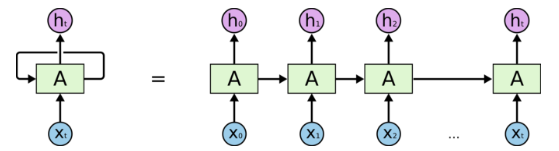
\includegraphics[width=0.9 \linewidth]{fig/rnn.png}
	\caption{An unrolled recurrent neural network. "A" is a recurrent unit (LSTM or GRU), $x_t$ is the input content and $h_t$ is the state output that is also used in the next computation round of the current state.}
	\label{fig:rnn}
\end{figure}
%\begin{itemize}
%	\item[(F1)] $CT$: cross term of two features $x_i$ and $x_j$, i.e., $x_i x_j$.
%	\item[(F2)] $\sqrt{CT}$: root square of the cross term.
%	\item[(F3)] $\arctan(CT)$: arctangent of the cross term.
%	\item[(F4)] $\sin(CT)$: sine of the cross term.
%	\item[(F5)] $CT^2$: square of the cross term
%\end{itemize}

We have implemented two common forms of recurrent layers, namely gated recurrent units and long short-term memory.
\subsubsection{Long Short-Term Memory}
LSTM’s have a Nature of Remembering information for a long periods of time in their Default behaviour. Therefore they help to extract dependencies between further words within a document. They consist of three gate called forget gate, input gate and output gate. Forget gate decides how much of the past should be remembered. Input gate decides how much of the current LSTM unit should be added to the current state and output gate decides which part of the current unit makes it to the output (which will be fed to the next LSTM layer). 

In addition to the aforementioned advantage, they also help to overcome the vanishing gradient issue which is a common issue with RNNs.

\subsubsection{Gated recurrent neural network}
Gated Recurrent Unit aims to solve the vanishing gradient problem which comes with a standard recurrent neural network. GRU can also be considered as a variation on the LSTM as they are both designed in a similar fashion. GRU consists of two main gates, namely the update gate and the reset gate. The former helps the model to determine how much of the past information (from previous time steps) needs to be passed along to the future and the latter is used to decide how much of the past information to forget. 
\section{Results \& Discussion} \label{sec:results}
Lots of classification schemes are tested throughout this project. First, to have an estimation about the baseline, simple classifiers including SVM and Logistic regression are implemented. Table \ref{tab:baseline_accuracy} shows the accuracy for these two methods.
\begin{table}[h]
	\centering
	\caption{Experimental results of baseline methods using tf-idf input.}
	\begin{tabular}{|c||c|}
		\hline
		Model &Accuracy\\
		\hline
		Support Vector Machine&  $77.8$\% \\ 
		\hline
		Regularized Logistic Regression&  $78.4$\% \\ 
		\hline
	\end{tabular}
	\label{tab:baseline_accuracy}
\end{table}

In order to improve our classification in terms of accuracy, three deep learning architectures (CNN, GRU, and LSTM) are implemented. For feature representation, GloVe embedding with $100$ dimensions, trained on almost two billion tweets is used. In all three schemes, we enable the back-propagation parameters to trained our architectures more accurately. All networks are trained for five epochs and the one with the best validation accuracy considered to be the train model. A convolutional neural network (describe in Section \ref{sec:conv}) leads to the accuracy of $82$\%, while with GRU neural network (see Section \ref{sec:RNN}) we are able to get the accuracy of more that $85$\%. Finally, the best accuracy is obtained with LSTM method (explained in …) with the accuracy of more than $86$\%.
\begin{table}[h]
	\centering
	\caption{Experimental results of deep learning methods using GloVe embedding with $100$ dimensions.}
	\begin{tabular}{|c||c|}
		\hline
		Model &Accuracy\\
		\hline
		Convolutional Neural Network&  $82$\% \\ 
		\hline
		Gated Recurrent Unit&  $85.6$\% \\ 
		\hline
		Long Short-Term Memory&  $86.2$\% \\ 
		\hline
	\end{tabular}
	\label{tab:deeplearning_accuracy}
\end{table}

At the end of previous step, we chose LSTM as the best training architecture. Then, we study the effects of using different feature vector dimension of GloVe. To do so, we trained our model with GloVe embeddings of $25$, $50$, $100$, and $200$ dimensions, that are trained on almost two billion tweets. Then, we also performed training with the GloVe embeddings with $300$ dimensions, trained on Common Crawl data-set containing about $2.2$ Million different vocabulary. 

\begin{table}[h]
	\centering
	\caption{Experimental results of LSTM using GloVe embedding with various dimensions.}
	\begin{tabular}{|c||c|}
		\hline
		GloVe dimension &Accuracy\\
		\hline
		$25$ &  $86$\% \\ 
		\hline
		$50$ &  $86.2$\% \\ 
		\hline
		$100$ &  $86.2$\% \\ 
		\hline
		$200$ &  $86.4$\% \\ 
		\hline
		\textbf{$300$} &  \textbf{$86.6$\%} \\ 
		\hline
	\end{tabular}
	\label{tab:lstm_accuracy}
\end{table}

Table \ref{tab:lstm_accuracy} reveals that although by increasing the dimensions of feature vector, more parameters need to be learned, we are able to get more powerful and accurate learning architecture for sentiment analysis.

%\begin{table}[t]
%	\centering
%	\caption{Experimental results of using different deep learning and baseline methods.}
%	\begin{tabular}{|c|c|c|c|c|}
%		\hline
%		\multirow{2}{*}{Model} &\multicolumn{3}{|c|}{Accuracy of GloVe dimensions} \\
%		\cline{2-4}
%	 										& dim=$25$ &dim=$50$&dim=$300$\\
%		\hline
%		LSTM & $1$\%&$1$\%&$1$\%\\
%		\hline
%		CNN &  $1$\% &$1$\%&$1$\%\\
%		\hline
%		GRU &  $1$\% &$1$\%&$1$\%\\
%		\hline
%		SVM&  $1$\% &$1$\%&$1$\%\\ 
%		\hline
%		RLR&  $1$\% &$1$\%&$1$\%\\ 
%		\hline
%	\end{tabular}
%	\label{tab:6model_accuracy}
%\end{table}
%Table~\ref{tab:results} shows the incremental results of this project using regularized logistic regression with cross validation. The execution of cross validation for the $8$ sub-datasets results in finding $n=2$ and $\lambda=10^{-20}$ for each one. 
%%Using these two parameters leads to a significant improvement in the accuracy of the prediction which is illustrated in Table \ref{tab:results}.
%
%Due to space limitation, we did not put some intermediate results and tried to show the effect of manual feature augmentation described in Subsection \ref{sec:man_feature}. The last row shows the expected accuracy of the model over the test data set by calculation of weighted average based on the size of each data-subset.
%
%Our observation shows that adding each of the functions (F1) to (F4), beside the polynomial expansion, leads to an improvement in the predictions. However, addition of (F5)  just improves the prediction in two sub-datasets with number of jets equal to $2$ and $3$ and the estimated mass is \textit{NA}. The column \textit{Final} in Table~\ref{tab:results} shows the final results that utilize (F1) to (F4) for all sub-datasets and also (F5) for the aforementioned sub-datasets. The \textit{Imp.} column shows the amount of improvement in comparison with the original features (no polynomial and manual feature augmentation). We submitted the final predictions in the aicrowd.com with the team \textit{Panda\_feat\_Ah}, and obtained $83.7$\% accuracy and F1-score of $0.754$.
%
%We have to mention that the same procedure is done using 10-fold ridge regression. Although the local predictions show high accuracy, the result of the prediction over the test dataset was by far worse than the one with regularized logistic regression.


\section{Conclusion} \label{sec:conclusion}

For the implementation we used Keras library in python.
%In this project, we applied regularized logistic regression to a binary classification problem in order to predict whether a particle is a signal or a background noise, based on some measured features. We also showed that data preprocessing helps to improve the results of a machine learning model by removing meaningless data. We figured out the significant effect of polynomial feature expansion and the cross validation. It is noteworthy to mention that manual addition of some functions to the model substantially increased the model accuracy. To wrap up, the polynomial expansion as well as the feature augmentation led to an average improvement of $13.89$\% in the local final prediction.

\bibliographystyle{IEEEtran}
\bibliography{library}

\end{document}
